\chapter{Design del frontend}
In questo capitolo ci soffermeremo sul design delle interfacce del frontend, utilizzando come riferimento dei wireframe creati con il web software \textbf{Balsamiq}.
L'interfaccia \`e suddivisa in due schermate principali, una per la gestione del Wallet e una per la gestione dei listini prezzi.

\section{Sezione per la gestione del Wallet}
Per monitorare il Wallet del suo tenant di appartenenza, l'utente ha a disposizione una dashboard in cui pu\`o visualizzare lo storico delle transazioni ed effettuare una ricarica del credito.

\begin{figure}[H]
  \centering
  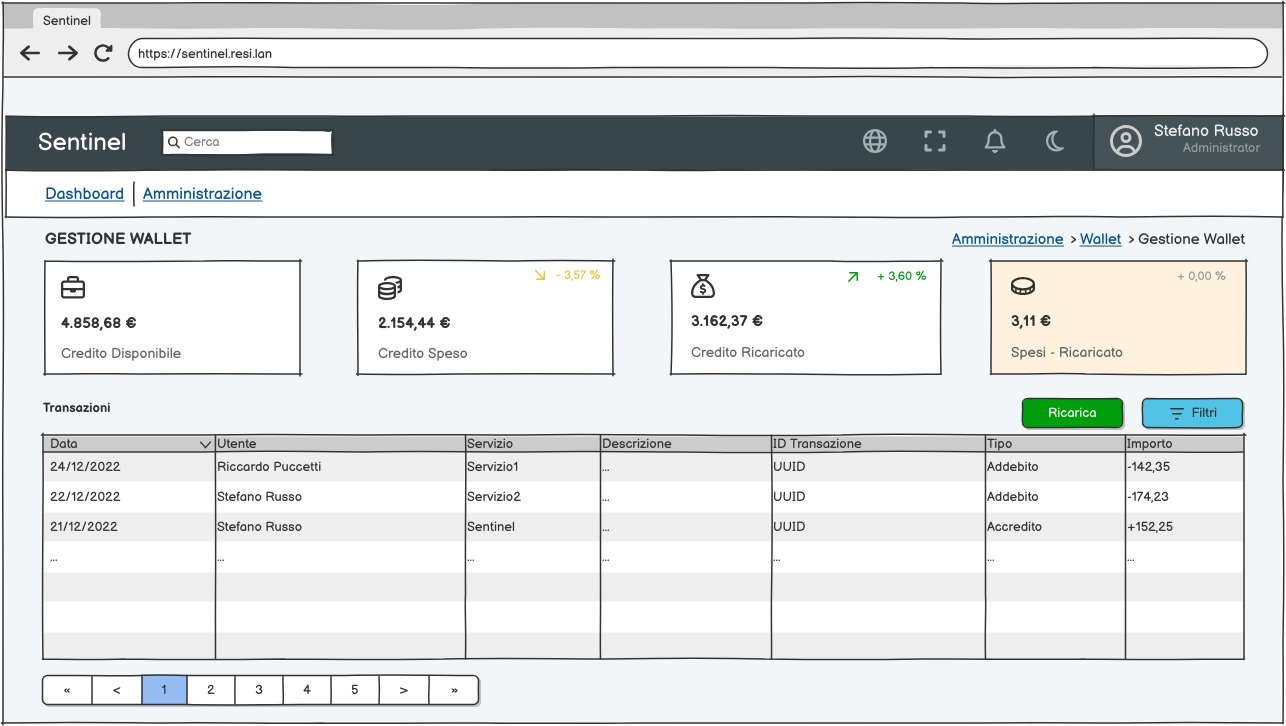
\includegraphics[width=13cm]{images/gestione-wallet/mock-gestione-wallet.png}
  \caption{Wireframe della schermata di Gestione Wallet}
\end{figure}

Nella parte superiore sono presenti dei widget che riportano alcune informazioni in modo da essere facilmente accessibili:
\begin{enumerate}
  \item Credito disponibile
  \item Credito speso  nel mese corrente
  \item Credito depositato nel mese corrente
  \item Differenza tra credito speso e credito depositato nel mese corrente
\end{enumerate}
Gli ultimi tre grafici riportano anche l'andamento rispetto al mese precedente.
\\\\
Il bottone \textbf{Ricarica} apre una schermata che permette di caricare un importo arbitrario, con la possibilit\`a di scegliere
dei tagli prestabiliti.

\begin{figure}[H]
  \centering
  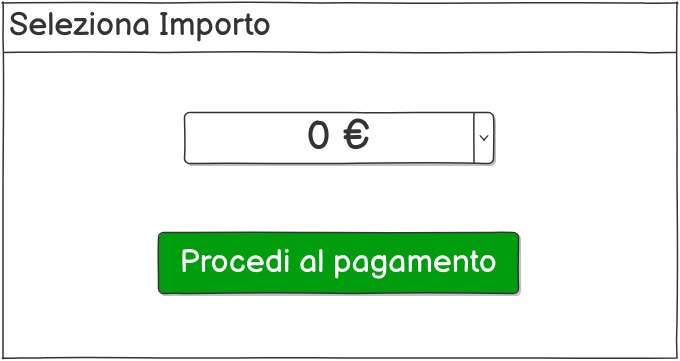
\includegraphics[width=8.5cm]{images/gestione-wallet/mock-seleziona-importo.png}
  \caption{Wireframe della schermata di selezione importo }
\end{figure}
Procedendo al pagamento si conferma l'importo, passando quindi alla schermata di pagamento di Stripe.

\begin{figure}[H]
  \centering
  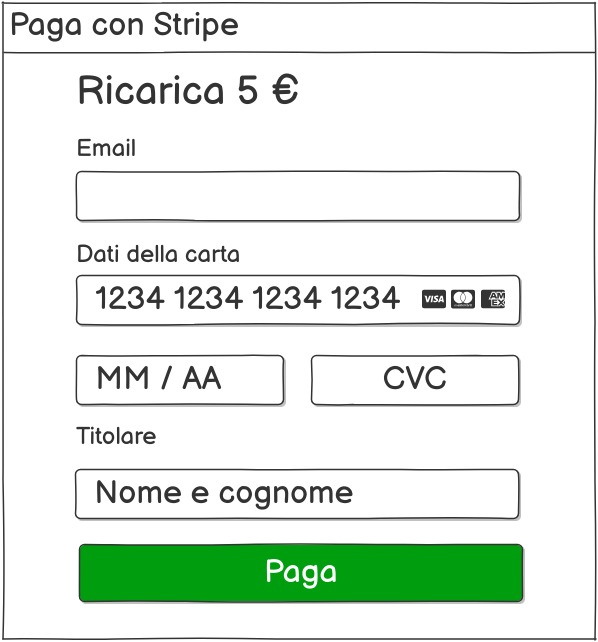
\includegraphics[width=5.5cm]{images/gestione-wallet/mock-stripe.png}
  \caption{Wireframe della schermata di pagamento con Stripe }
\end{figure}

Il bottone \textbf{Filtri} apre una schermata laterale dove \`e possibile selezionare le propriet\`a per cui deve essere filtrata la lista delle transazioni.

\begin{figure}[H]
  \centering
  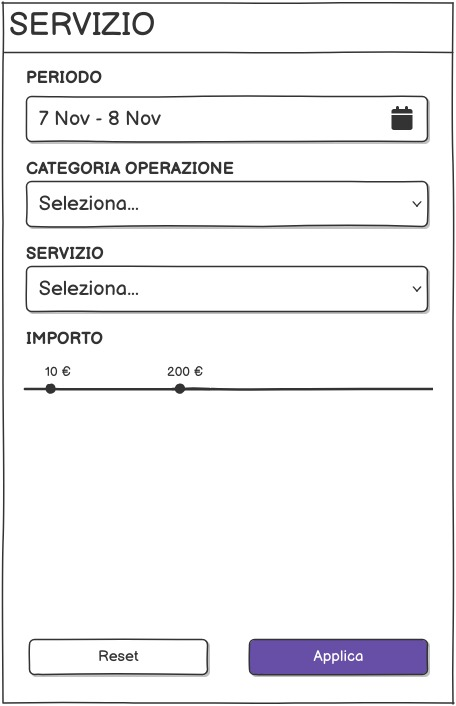
\includegraphics[width=6cm]{images/gestione-wallet/mock-filtri-ricerca.png}
  \caption{Wireframe della schermata dei filtri}
\end{figure}

\section{Sezione per la gestione dei listini prezzi}
L'amministratore ha a disposizione una schermata in cui pu\`o aggiungere, modificare o cancellare un listino prezzi, come indicato nella \textbf{Figura \ref{listalistini}}.
\begin{figure}[H]
  \centering
  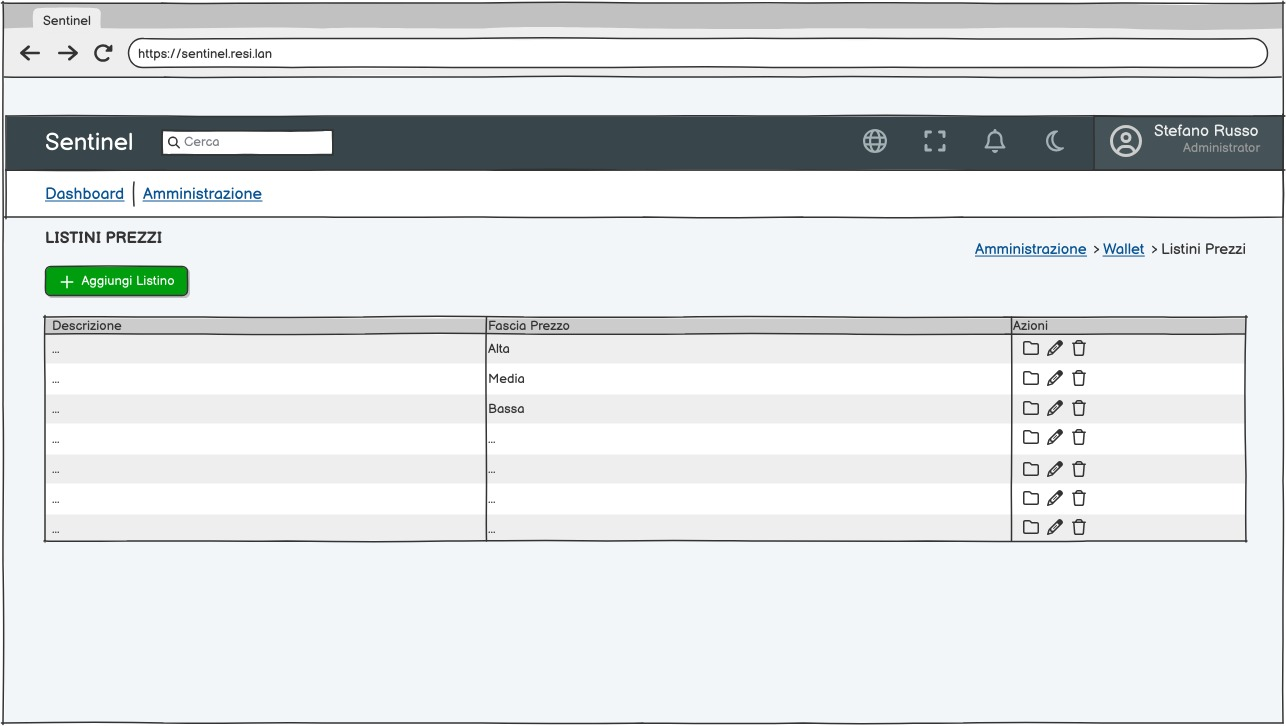
\includegraphics[width=13cm]{images/gestione-listini/listini-prezzi-list.png}
  \caption{Wireframe della schermata con la lista dei listini prezzi}
  \label{listalistini}
\end{figure}
Il bottone \textbf{Aggiungi Listino} reindirizza a una pagina che consente di inserire i dati per creare un nuovo listino prezzi, come nella \textbf{Figura \ref{aggiungilistino}}.
\\\\
Nella tabella invece sono presenti 3 azioni per ogni listino prezzi:
\begin{enumerate}
  \item Apertura del dettaglio come indicato nella \textbf{Figura \ref{dettagliolistino}}.
  \item Reindirizzamento a una pagina analoga a quella della \textbf{Figura \ref{aggiungilistino}}, che permette di modificare il listino prezzi.
  \item Apertura di una schermata di conferma per l'eliminazione del listino.
\end{enumerate}

\begin{figure}[H]
  \centering
  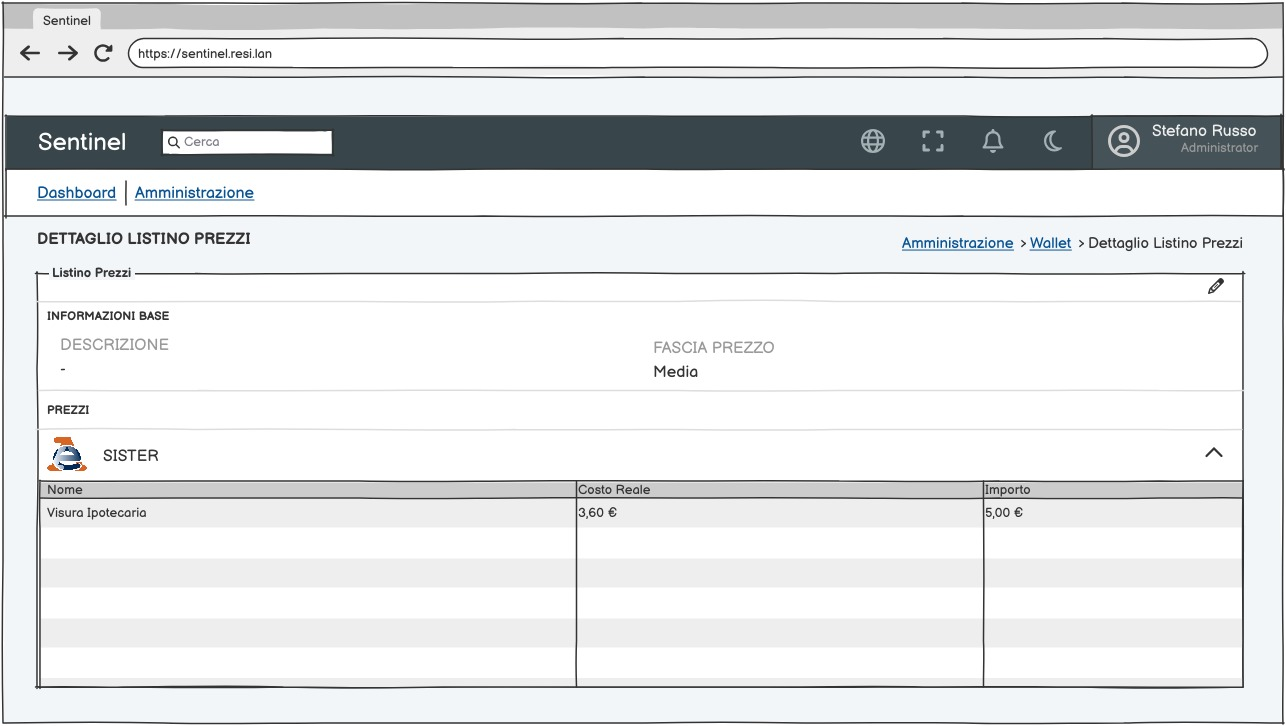
\includegraphics[width=13cm]{images/gestione-listini/dettaglio-listino.png}
  \caption{Wireframe della schermata del dettaglio di un listino prezzi}
  \label{dettagliolistino}
\end{figure}

Il dettaglio del listino prezzi \`e suddiviso in due sezioni: nella sezione \textbf{Informazioni Base} sono presenti la descrizione e la fascia di prezzo, mentre nella sezione
\textbf{Prezzi} \`e presente una tabella nascondibile per ogni banca dati, con il relativo costo di ogni operazione all'interno del listino prezzi.
Con il bottone di edit (l'icona a forma di matita) si viene reindirizzati a una pagina che permette di modificare il listino, analoga alla schermata presente nella \textbf{Figura \ref{aggiungilistino}}.

\begin{figure}[H]
  \centering
  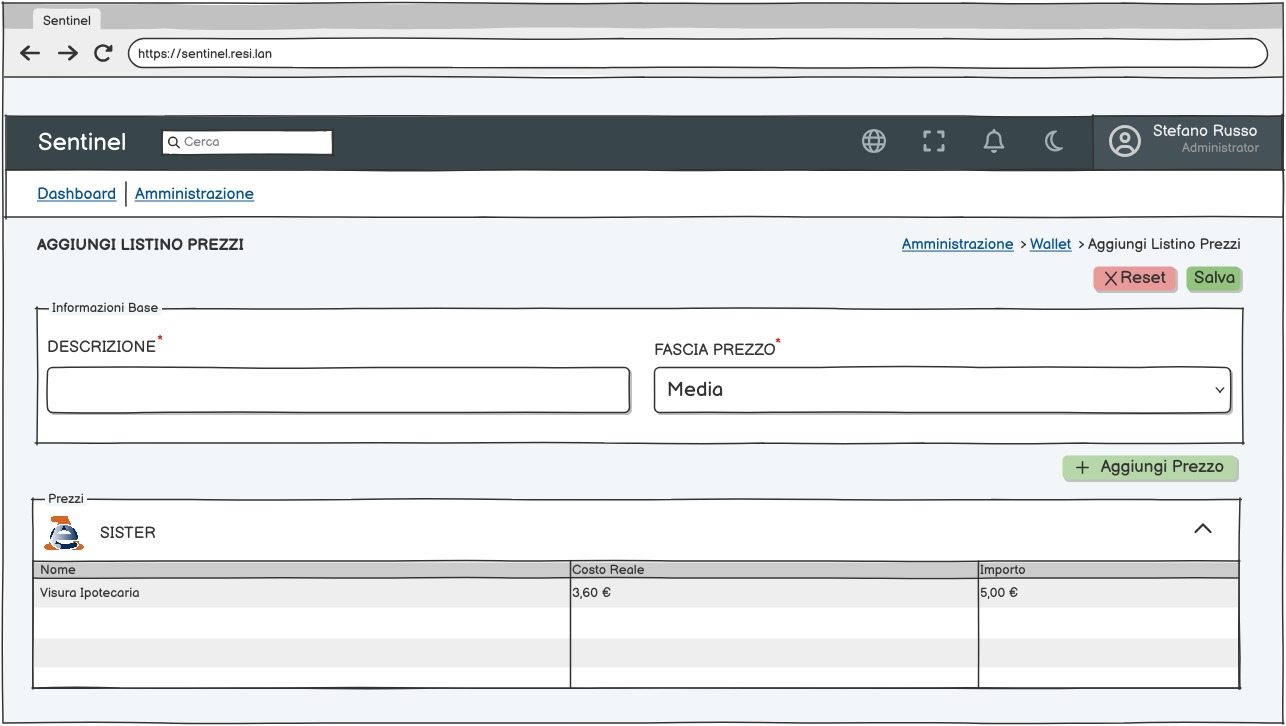
\includegraphics[width=13cm]{images/gestione-listini/add-listino.png}
  \caption{Wireframe della schermata di creazione listino prezzi}
  \label{aggiungilistino}
\end{figure}
Nella sezione \textbf{Informazioni Base} \`e possibile inserire una descrizione e una fascia di prezzo.
Nella sezione \textbf{Prezzi} \`e presente una tabella nascondibile per ogni banca dati che riporta i costi inseriti.
Cliccare su una riga apre una schermata analoga a quella indicata nella \textbf{Figura \ref{aggiungiprezzo}}, con la differenza che la selezione del tipo operazione
non \`e presente, in quanto il campo \`e preselezionato. Questa schermata consente quindi di modificare il prezzo inserito in precedenza.

Per terminare la creazione di un Listino \`e necessario inserire un importo per tutte le operazioni di pagamento.
\\\\
Il bottone \textbf{Aggiungi Prezzo} apre la schermata di aggiunta del prezzo in \textbf{Figura \ref{aggiungiprezzo}}
\begin{figure}[H]
  \centering
  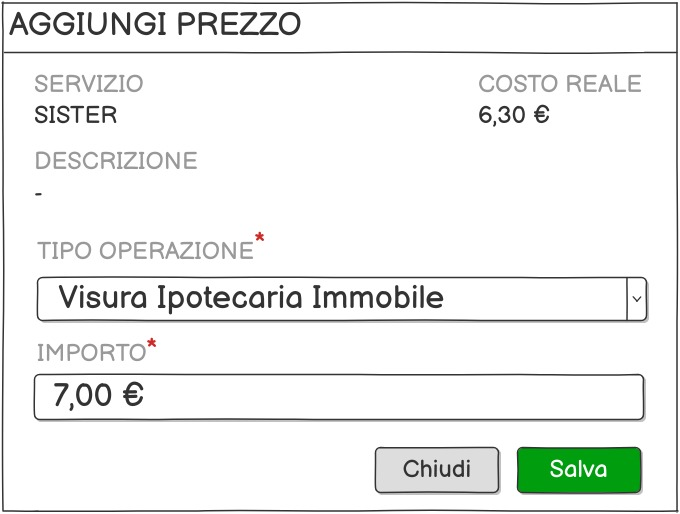
\includegraphics[width=8.5cm]{images/gestione-listini/aggiungi-prezzo.png}
  \caption{Wireframe della schermata per inserire un importo}
  \label{aggiungiprezzo}
\end{figure}

Da questa schermata \`e possibile selezionare un tipo operazione e specificare il suo importo, potendolo sempre confrontare con il costo reale di interrogazione della banca dati esterna.
